\documentclass[11pt]{article}
\usepackage[margin=1in]{geometry}
\usepackage{booktabs,graphicx,microtype,caption,enumitem,xcolor,amsmath}
\usepackage[colorlinks=true,linkcolor=blue!50!black,citecolor=blue!50!black,urlcolor=blue!50!black]{hyperref}
\captionsetup{font=small,labelfont=bf}
\setlist{itemsep=2pt,topsep=4pt}
\graphicspath{{../figures/}}

\title{Moral judgement in a vision model that never saw a word\\[4pt]
\large Probing DINOv2 on the Socio-Moral Image Database. Technical report}
\author{Eli Ovits\\ \small\url{https://github.com/eliovi/moral_judgement_in_dinov2}}
\date{November 2026}

\begin{document}
\maketitle

\begin{abstract}
\noindent Language models represent a direction that separates morally good from bad actions, but they learn it from text in which people discuss right and wrong. We ask whether a vision model with no access to language learns the same thing. DINOv2 is trained on images alone, with no labels and no captions. We fit linear probes on its frozen features to predict human ratings of 2,940 photographs from the Socio-Moral Image Database. On held-out images the probe orders photographs by morality almost as people do (Spearman $\rho=0.74$). The signal is not explained by image statistics or object identity. It survives their removal, holds within groups of images that show the same kinds of objects, and transfers to object categories the probe never trained on. Part of it reflects morality beyond mere pleasantness: scenes of rescue and care rank as good even though they are unpleasant to look at. Read through a translation into CLIP's image--text space that never saw a rating, DINOv2's morality direction lines up with virtue words such as \emph{volunteering}, \emph{heroism} and \emph{respect}. This signal appears only in the last third of the network and grows with model size, while object information does not. Finally, CLIP, which learned from captions, and DINOv2, which did not, end up with nearly the same morality direction, and their agreement grows with depth and size. We read this as evidence that good versus bad is part of the structure that capable models of the visual world converge on, and we state the limits of a single-dataset probing study.
\end{abstract}

\section{Introduction}

Large language models can say whether an action is right or wrong, and their internal representations contain a direction that tracks this \cite{schramowski2022,zou2023}. That is not surprising. Their training text is full of people explaining what is good and bad. A model of images has no such teacher. If a vision model trained without labels or language still organises photographs along a good--bad axis that matches human judgement, the concept is learnable from how the world looks, and possibly something any capable model of the world ends up with.

The closest prior work is Zhu, Ramezani and Xu \cite{zhu2025}. They predicted the morality and moral-foundation ratings of the Socio-Moral Image Database (SMID) \cite{crone2018} with ridge regression on CLIP ViT-B/32 embeddings. Image embeddings did better than models of the image captions (average test $R^2$ of 0.63 against 0.43), and they used the predictor to study news photographs. CLIP, however, is trained on 400 million image--caption pairs \cite{radford2021}, so its moral signal could come from language. We remove language entirely and study DINOv2 \cite{oquab2023}, which is trained by self-distillation on images only.

The report follows the questions a sceptical reader would ask. Does DINOv2 carry the information at all (Test 1)? Is it using a shortcut such as dark images or particular objects (Test 2)? Is it morality, or only pleasantness (Test 3)? What does the direction mean in words (Test 4)? Where in the network does it appear, and does it grow with scale (Test 5)? And do models trained in completely different ways end up with the same direction (Test 6)?

\begin{figure}[ht]\centering
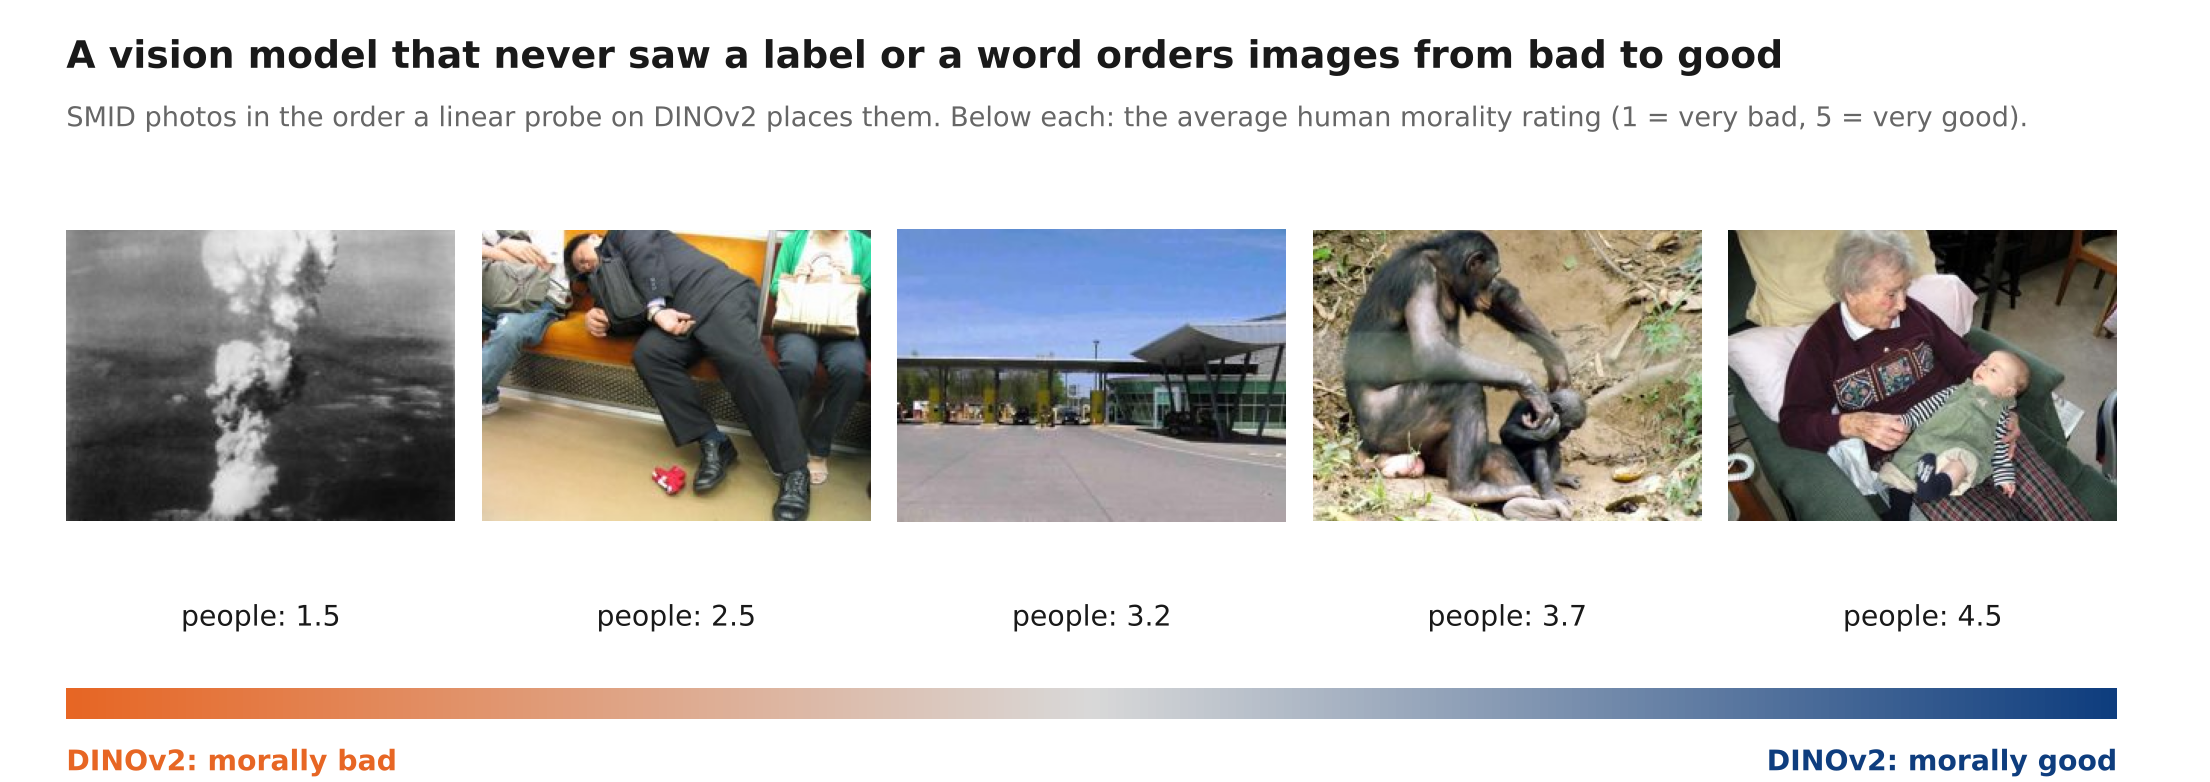
\includegraphics[width=\linewidth]{fig1_bad_to_good.png}
\caption{Five SMID photographs in the order a linear probe on DINOv2 places them. Numbers are the mean human morality rating (1 = very bad, 5 = very good).}\label{fig:strip}
\end{figure}

\section{Data and models}

\paragraph{SMID.} The Socio-Moral Image Database \cite{crone2018} contains 2,941 freely licensed photographs with positive, negative and neutral moral and emotional content. Its ratings come from more than 820,000 judgements by 2,716 participants, about 30 raters per image and scale. Each image has a mean rating on 1--5 scales for \emph{morality} (immoral to moral), \emph{valence} (unpleasant to pleasant) and arousal, plus relevance ratings for the five foundations of Moral Foundations Theory \cite{graham2013}, and a standard error for every mean. We use the 2,940 images that have all three main ratings. Across images, morality and valence are strongly related ($\rho=0.87$), which is why Test 3 is needed.

\paragraph{COCO.} The 5,000 photographs of COCO \texttt{val2017} \cite{lin2014}, without any annotation, are used only to learn translations between DINOv2 and CLIP. No SMID image or rating is involved.

\paragraph{DINOv2.} We use the four public models \cite{oquab2023}: ViT-S/14 (21M parameters, 12 layers), ViT-B/14 (86M, 12 layers), ViT-L/14 (300M, 24 layers) and ViT-g/14 (1.1B, 40 layers). The three smaller ones are distilled from ViT-g. Images are resized to 256 pixels and centre-cropped to 224. At each layer we represent an image by its CLS token concatenated with the average of its patch tokens. Unless stated otherwise we use ViT-g layer 37 of 40, the best layer for both ratings.

\paragraph{Reference models and control features.} CLIP ViT-L/14 \cite{radford2021} image embeddings serve as a language-trained comparison; text is embedded with the template ``a photo of \{\}''. For the shortcut tests we compute three sets of control features for every image:
\begin{itemize}
\item \emph{Low-level statistics} (57 numbers at $224\times224$): mean and spread of the RGB and HSV channels and of luminance, edge strength (gradient magnitude), a colourfulness index, the brightness of each image quadrant, and histograms of luminance (16 bins), saturation (8) and hue (12).
\item \emph{Object identity}: the 1,000 ImageNet \cite{deng2009} class scores (logits) of a supervised ViT-B/16 classifier \cite{dosovitskiy2021} (\texttt{google/vit-base-patch16-224}).
\item \emph{Supervised features}: the same classifier's final 768-dimensional embedding, which carries everything it learned from ImageNet labels, not only the class decision.
\end{itemize}

\section{Methods}

\paragraph{The probe.} A probe is a simple model trained to read a property out of frozen features. Ours is linear: the features are standardised, reduced to their first 256 principal components, and fed to a ridge regression that predicts the mean human rating. The ridge penalty is chosen among 13 values from $10^{-1}$ to $10^{5}$ by efficient leave-one-out cross-validation inside the training data. Because the model is linear, a good score means the rating lies along a direction in DINOv2's representation space; this direction is what we call DINOv2's ``morality direction''. A linear probe shows that information is present and easy to read, not that the network uses it \cite{alain2016,belinkov2022}.

\paragraph{Training and test data.} We never score an image with a probe that saw it. The 2,940 images are shuffled and split into 5 folds of 588. For each fold we fit the whole pipeline (standardisation, principal components, ridge penalty and weights) on the other 2,352 images and predict the 588 held-out ones. After the five rounds every image has exactly one prediction made without it, its \emph{out-of-fold} prediction, and all metrics are computed on these. Test 2d uses the same procedure, but folds are formed from whole groups of images with similar objects, so the test images show object categories absent from training.

\paragraph{Metrics.} The main metric is Spearman's rank correlation $\rho$ between the out-of-fold predictions and the mean human ratings. It asks whether the probe puts the 2,940 images in the same order as people do: $\rho=1$ is the same order, $\rho=0$ is no relation. We use ranks because the ratings are bounded averages and the order is what matters. For a second, more intuitive view we also report the AUROC for separating the top third of images from the bottom third. We draw 300 images from each, train a probe to tell them apart with 5-fold cross-validation, and measure the probability that a random top-third image receives a higher score than a random bottom-third one (0.5 is chance, 1 is perfect). The 95\% confidence intervals come from resampling the images with replacement (300 to 1,000 times) and recomputing the metric.

\paragraph{Removing a possible shortcut.} To ask whether DINOv2 knows anything about a rating $y$ beyond a set of control features $Z$, we first predict $y$ from $Z$ and keep only what $Z$ cannot explain, the residual $r = y - \hat{y}_Z$. We then probe DINOv2 for $r$. If DINOv2 predicts $r$, it carries information about the rating that the controls do not. The prediction $\hat{y}_Z$ is itself out-of-fold. Otherwise a flexible control could memorise the ratings and remove signal that has nothing to do with it. We use two kinds of control model:
\begin{itemize}
\item A \emph{linear control} is the same pipeline as the probe (standardise, 256 principal components, ridge) trained on the control features. It removes everything that is a weighted sum of the controls.
\item A \emph{non-linear control} can also remove information that only a non-linear function of the controls carries, for example ``a gun next to a child''. We use two. $k$-nearest-neighbour regression predicts each image's rating as the distance-weighted average rating of the 25 most similar images in control-feature space. Gradient-boosted regression trees use 300 trees with learning rate 0.05. Both work on the first 64 principal components of all control features together. The strictest version stacks them: first the linear control, then the average of the $k$-NN and boosted predictions fitted to what the linear control left.
\end{itemize}

\paragraph{Permutation test.} For the weakest result (Section~\ref{sec:mbv}) we shuffle the target ratings across images 200 times and rerun the probe each time. This gives the scores a probe reaches when there is nothing to find. Standardisation and principal components do not depend on the target, so they are kept fixed and only the ridge is refitted.

\paragraph{Translating between models.} Embedding spaces of different models can often be mapped onto each other \cite{jha2025,tasker2026}. We use the simplest version: pass the same images through both models and fit a linear map (standardise, principal components, multi-output ridge) from one embedding to the other. Sections~\ref{sec:words} and~\ref{sec:shared} describe which images each map is fitted on.

\section{Test 1: Does DINOv2 carry the information?}

We probed every second layer, plus the last, of all four DINOv2 sizes. All three ratings are predicted well (Table~\ref{tab:base}). The largest model orders images by morality at $\rho=0.74$ and separates the most and least moral thirds with AUROC 0.94. In every size the best layer is in the last 10\% of the network. These raw numbers alone prove little: a probe could be reading darkness, objects or pleasantness. The next two tests address that.

\begin{table}[ht]\centering\small
\begin{tabular}{lcccc}\toprule
 & ViT-S & ViT-B & ViT-L & ViT-g\\\midrule
Morality, $\rho$ & 0.646 & 0.700 & 0.726 & 0.743\\
Valence, $\rho$ & 0.695 & 0.730 & 0.748 & 0.762\\
Arousal, $\rho$ & 0.661 & 0.697 & 0.719 & 0.724\\
Morality, AUROC top vs bottom third & 0.888 & 0.912 & 0.930 & 0.936\\
Valence, AUROC top vs bottom third & 0.895 & 0.913 & 0.933 & 0.938\\\bottomrule
\end{tabular}
\caption{Best-layer probe performance on held-out images, by DINOv2 size.}\label{tab:base}
\end{table}

\section{Test 2: Is it a shortcut?}\label{sec:shortcuts}

Photographs of bad events may simply be darker or greyer, or contain particular objects such as weapons or children. We test both explanations, first with linear controls, then with non-linear ones, and finally with two tests that do not rely on removing anything.

\paragraph{2a. Linear controls.} We remove, one set at a time, what the low-level statistics, then also the ImageNet class scores, then also the supervised features can predict (Table~\ref{tab:controls}, Figure~\ref{fig:controls}). Image statistics barely matter: morality goes from 0.74 to 0.70. Objects matter much more, but after all three controls DINOv2 still predicts morality at 0.32 and valence at 0.36. CLIP, shown for reference, keeps more (0.60 and 0.65).

\begin{table}[ht]\centering\small
\begin{tabular}{lccc}\toprule
Controls removed & Morality & Valence & Morality beyond valence\\\midrule
none & 0.735 & 0.761 & 0.609\\
low-level statistics & 0.699 \,(0.68--0.72) & 0.718 \,(0.70--0.74) & 0.579 \,(0.55--0.60)\\
+ ImageNet class scores & 0.352 \,(0.32--0.38) & 0.382 \,(0.35--0.41) & 0.191 \,(0.16--0.23)\\
+ supervised features & 0.321 \,(0.29--0.35) & 0.356 \,(0.32--0.39) & 0.163 \,(0.13--0.20)\\\midrule
\emph{controls alone predict the rating at} & \emph{0.664} & \emph{0.689} & \emph{0.563}\\\bottomrule
\end{tabular}
\caption{DINOv2-g (layer 37) on the part of each rating the controls do not explain. Spearman $\rho$ with 95\% confidence interval. ``Morality beyond valence'' is defined in Section~\ref{sec:mbv}.}\label{tab:controls}
\end{table}

\begin{figure}[ht]\centering
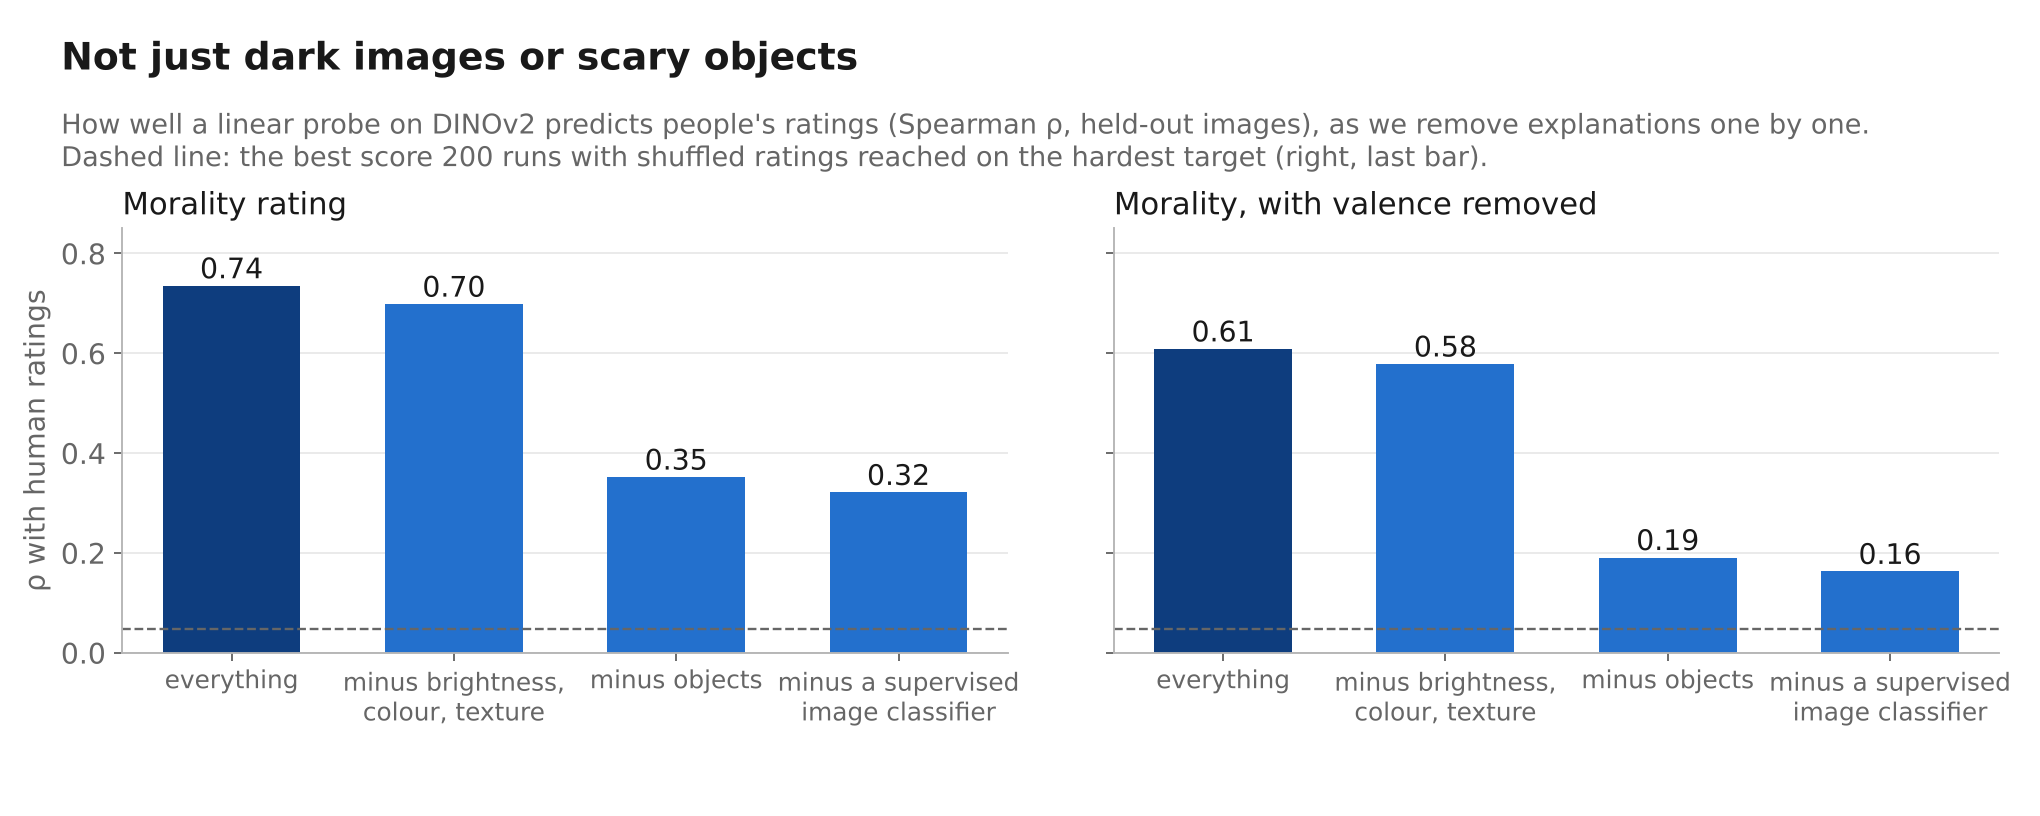
\includegraphics[width=0.95\linewidth]{fig2_controls.png}
\caption{DINOv2's prediction of the morality rating (left) and of morality beyond valence (right) as shortcuts are removed one at a time.}\label{fig:controls}
\end{figure}

\paragraph{2b. Non-linear controls.} Used alone, the $k$-NN and boosted controls remove less than the linear one (DINOv2 keeps 0.51 and 0.38 for morality). The stacked control is the strictest test in this report. After it, DINOv2 still predicts morality at 0.20 (0.16--0.23) and valence at 0.23 (0.20--0.27). Morality beyond valence, however, drops to 0.03 (from $-0.002$ to 0.07), which is not significant, while CLIP keeps 0.29. This control also removes real signal, since the supervised classifier inside it predicts morality beyond valence at 0.58 by itself.

\paragraph{2c. Same objects, different rating.} If DINOv2 only knew object categories, it could not rank images that show the same kinds of things. We grouped the images into $K=50$ and $K=150$ clusters by their control features ($k$-means on the 64 principal components), removed each cluster's average from both the ratings and the predictions (working on ranks), and correlated what was left. Cluster membership explains only 20--37\% of the variance of the ratings. Within clusters ($K=50$) DINOv2 ranks morality at 0.65 (0.61--0.67) and valence at 0.67 (0.64--0.69), above a probe on the control features themselves (0.53 and 0.55). Here the confidence intervals resample whole clusters.

\paragraph{2d. Object categories never seen in training.} We grouped images into 50 clusters by their ImageNet class scores alone and used grouped cross-validation, so each test fold contains only object groups absent from its training data. If the probe had memorised which objects are good or bad, it would fail. It does not: morality drops only from 0.74 to 0.70, valence from 0.76 to 0.74, and morality beyond valence from 0.61 to 0.57. A probe on the class scores themselves reaches 0.56, 0.59 and 0.47 under the same split.

\section{Test 3: Morality, or only pleasantness?}\label{sec:mbv}

With morality and valence correlated at 0.87, a probe could read ``pleasant versus unpleasant'' and get morality nearly for free. To isolate the moral part we define \emph{morality beyond valence} (MBV): the morality rating minus what a smooth function of valence predicts (a cubic spline with 8 knots, fitted by ridge regression). MBV holds 23\% of the variance of the morality rating and is unrelated to valence ($\rho=0.03$). Removing valence with a straight line instead, or removing arousal as well, changes DINOv2's result by less than 0.03.

\paragraph{How much is noise?} Each SMID rating is an average of about 30 people, so it comes with a standard error. The reliability of a target is the share of its variance that is not rating noise, $1-\overline{\mathrm{SE}^2}/\mathrm{Var}(y)$; for MBV we combine the errors of both ratings through the local slope of the spline, assuming they are independent. Reliability is 0.97 for valence, 0.95 for morality, 0.70 for MBV and 0.55 for MBV after the controls of Table~\ref{tab:controls}. The last value implies that even a perfect predictor could reach only about $\rho=0.74$ on that target (0.38 if the two rating errors were fully correlated).

\paragraph{Is it significant?} Without controls DINOv2 predicts MBV at 0.61. After the controls it predicts it at $\rho=0.163$ (0.13--0.20). In 200 runs on shuffled ratings the probe averaged $-0.004$ (standard deviation 0.026) and never exceeded 0.048, so the observed value is 6.5 standard deviations above chance ($p<0.005$). On the half of images with the most precise morality ratings the correlation is 0.19, on the other half 0.14, as expected for a real signal blurred by noise.

\paragraph{What is in it?} MBV correlates with every moral-foundation relevance rating (harm 0.44, fairness 0.36, ingroup 0.47, authority 0.53, purity 0.38) and not with arousal (0.09). The raw morality rating relates to these weakly or not at all. The images DINOv2 scores highest and lowest on MBV, where people agree, show the distinction: unpleasant scenes of rescue, care and duty, against pleasant scenes with little moral content (Figure~\ref{fig:offdiag}).

\begin{figure}[ht]\centering
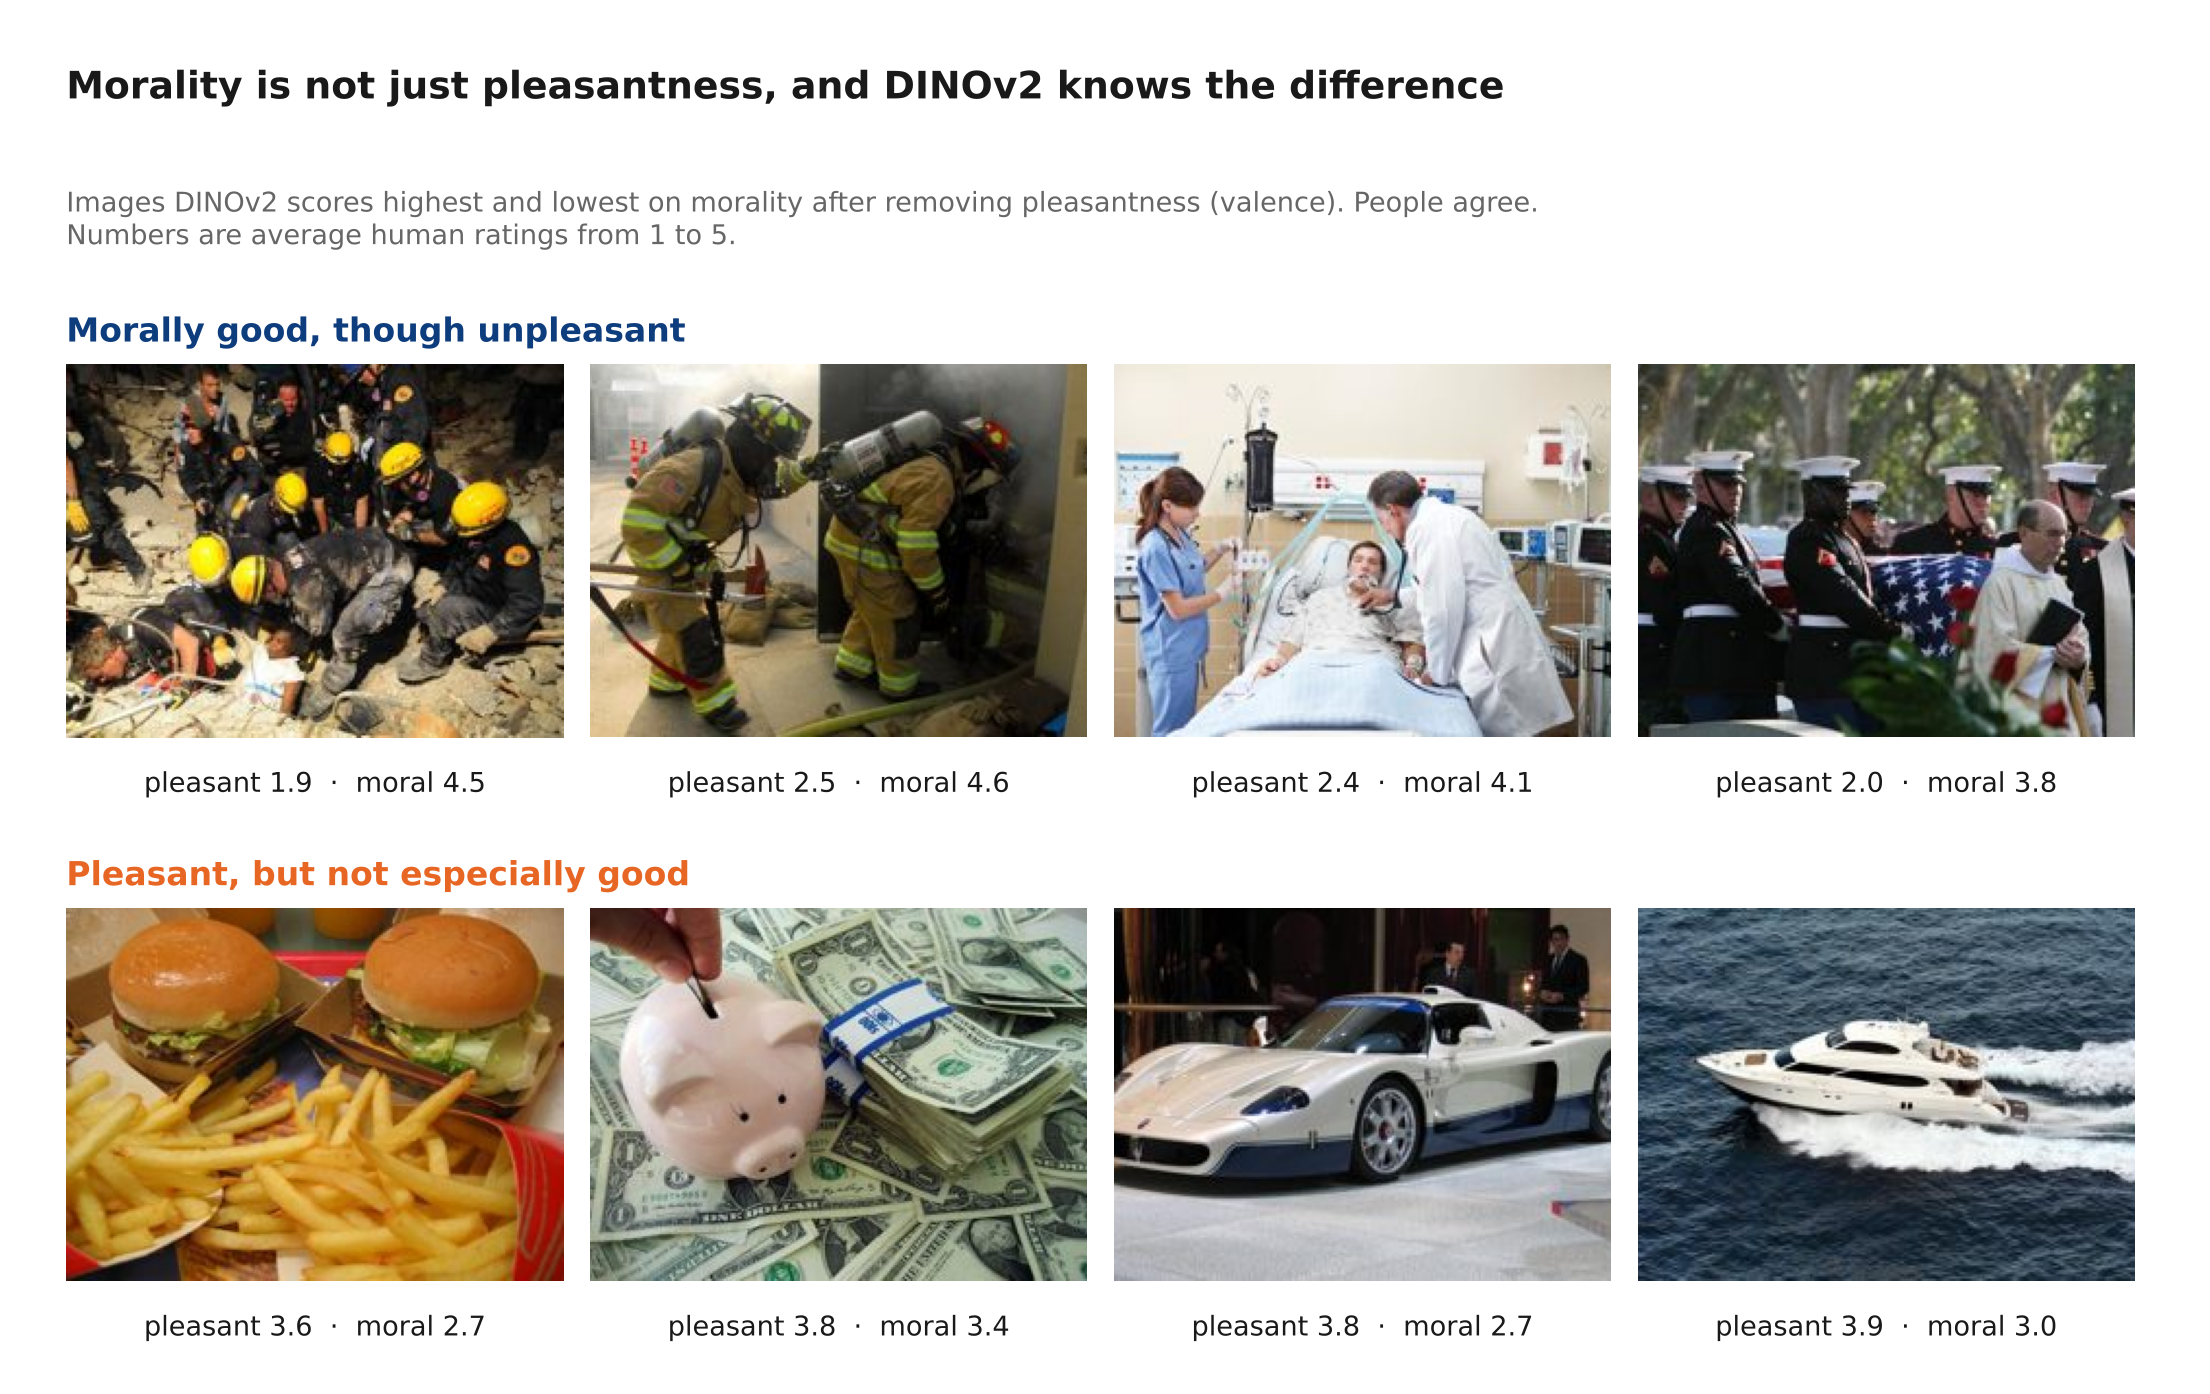
\includegraphics[width=0.92\linewidth]{fig3_beyond_pleasant.png}
\caption{Images with the highest and lowest DINOv2-predicted morality beyond valence, among images where the human ratings agree. Numbers are mean human ratings (1--5).}\label{fig:offdiag}
\end{figure}

\section{Test 4: What the direction means, in words}\label{sec:words}

The probe direction is a vector of numbers. To check that it is about morality, and not a quirk of the ratings, we read it in language, through a translation that never sees a rating.

\paragraph{The translation.} We passed the 5,000 COCO photographs through DINOv2-g (layer 37) and CLIP, and fitted a linear map from DINOv2's embedding of each photo to CLIP's embedding of the same photo (256 principal components, multi-output ridge). We then applied the map, unchanged, to the SMID images. The translation is reasonable. A probe on the translated embeddings still predicts valence at $\rho=0.72$. With a 512-component version of the map, a translated image's nearest neighbour among all 2,940 real CLIP embeddings is its own 36\% of the time (in the top five, 58\%). Its average cosine similarity to its own CLIP embedding is 0.77, against 0.59 for a random image.

\paragraph{Reading the direction.} We fixed a vocabulary of 150 terms in advance, in five groups: 30 virtues (\emph{kindness, fairness, helping others, heroism}, \dots), 30 vices (\emph{cruelty, theft, vandalism}, \dots), 20 positive-emotion terms (\emph{joy, fun, beauty, a party}, \dots), 20 negative-emotion terms (\emph{sadness, pain, decay}, \dots) and 50 everyday things (\emph{a dog, a car, a phone, a hospital}, \dots). For each term, and across all SMID images, we correlated two quantities. One is how similar the translated image is to ``a photo of $\langle$term$\rangle$''. The other is DINOv2's own out-of-fold score. Terms with a high correlation are what DINOv2's high-scoring images look like, in CLIP's terms. To compare groups we use an AUC: the probability that a random term from one group ranks above a random term from another.

\paragraph{Result.} The morality direction prefers virtues to vices (AUC 0.83). Its top terms include \emph{fairness, volunteering, helping others}, and its bottom terms \emph{decay, poverty, neglect, vandalism}. The direction for morality beyond valence prefers virtues to merely pleasant words (AUC 0.84). Its top terms are \emph{volunteering, helping others, heroism, cooperation, respect, gratitude, fairness}, and its bottom terms \emph{beauty, a bird, a pizza, a cat, a phone, a dog}. For contrast, the valence direction prefers pleasant words to virtues (AUC 0.36 for virtue over positive emotion), as it should (Table~\ref{tab:words}, Figure~\ref{fig:words}). One top term is unexpected: \emph{slavery} is fifth for morality beyond valence, probably because of SMID's historical and memorial photographs.

\begin{table}[ht]\centering\small
\begin{tabular}{lccc}\toprule
Direction & virtue over vice & virtue over positive emotion & negative emotion over vice\\\midrule
Morality & 0.83 & 0.57 & 0.19\\
Morality beyond valence & 0.67 & 0.84 & 0.38\\
Valence (for contrast) & 0.81 & 0.36 & 0.25\\\bottomrule
\end{tabular}
\caption{How strongly each DINOv2 direction prefers one word group to another (AUC; 0.5 means no preference).}\label{tab:words}
\end{table}

\begin{figure}[ht]\centering
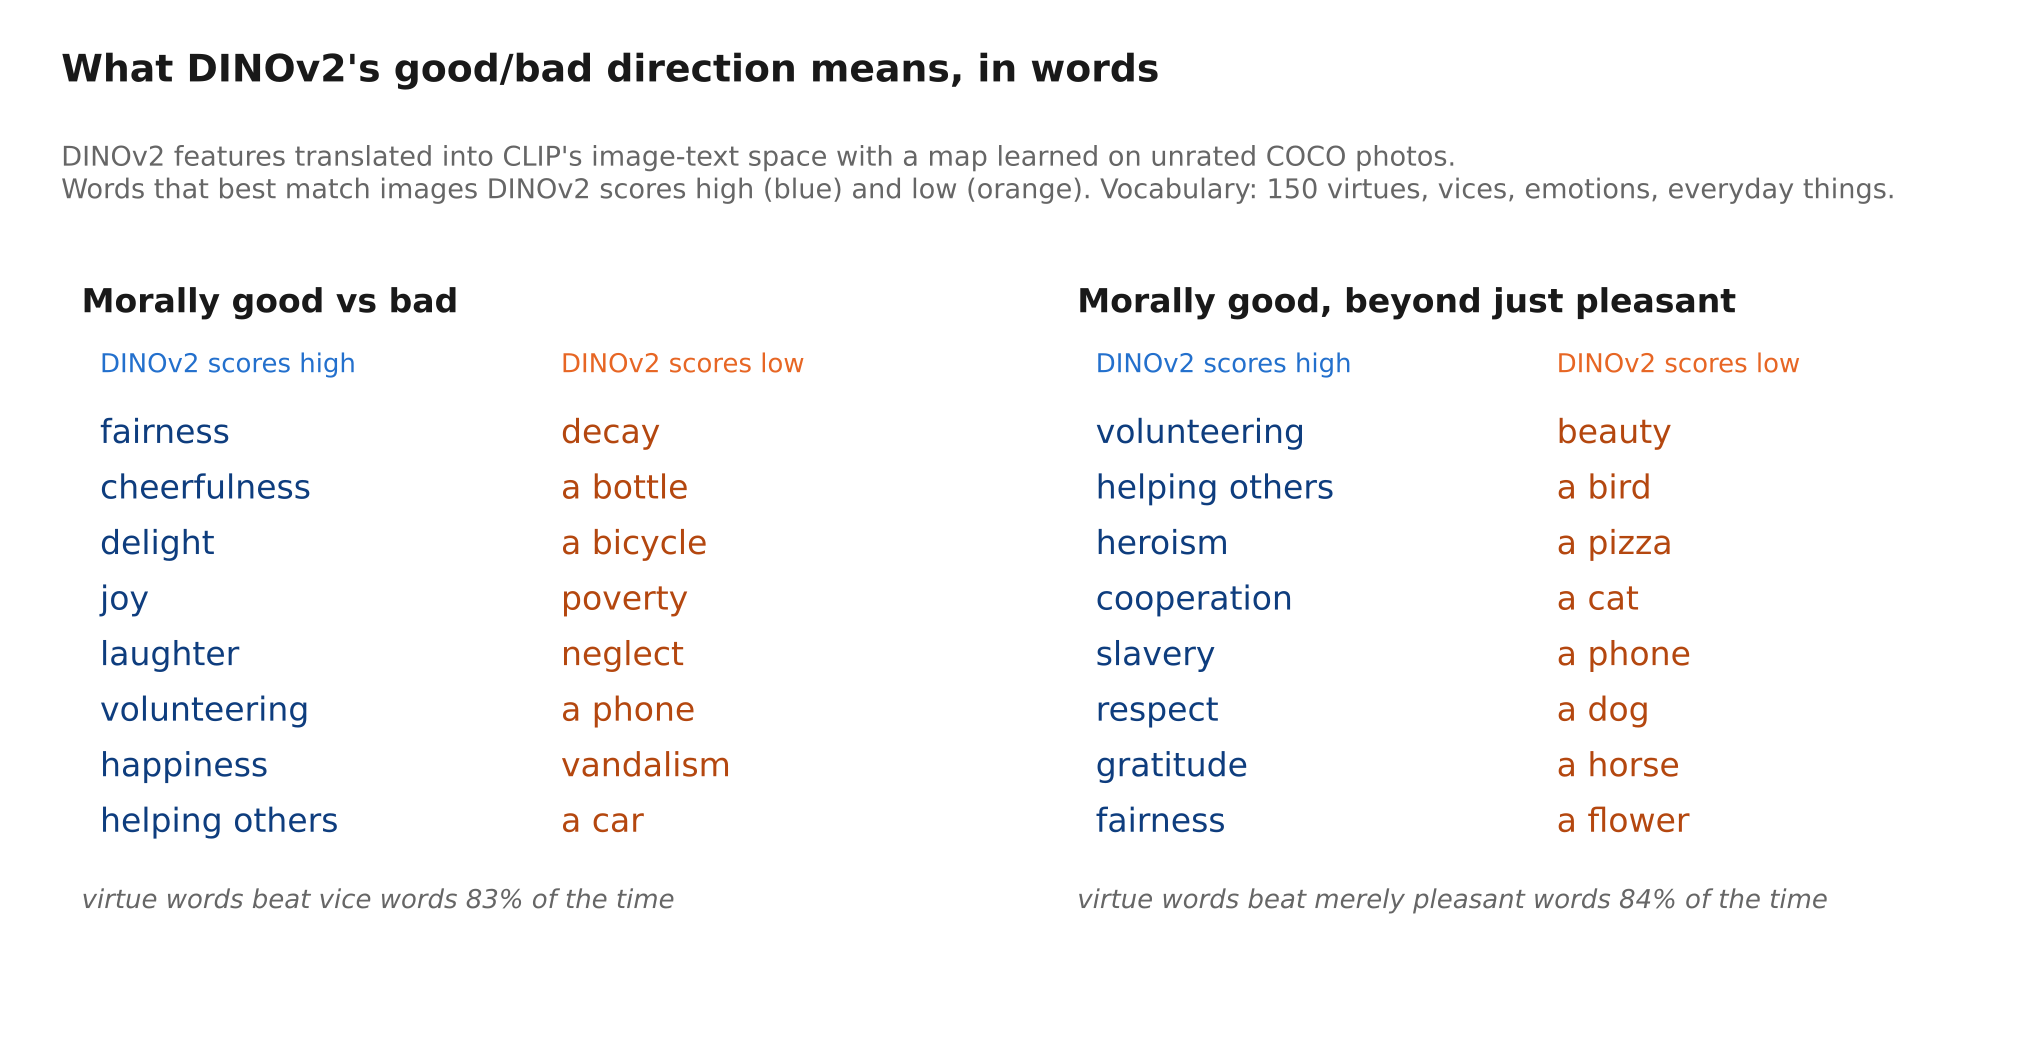
\includegraphics[width=0.9\linewidth]{fig4_words.png}
\caption{Top and bottom terms for DINOv2's morality direction and its morality-beyond-valence direction.}\label{fig:words}
\end{figure}

\section{Test 5: Where it appears, and how it scales}\label{sec:scale}

If good versus bad is a high-level abstraction, it should appear late in the network and benefit from more capacity, unlike low-level or object information. For each DINOv2 size we probed 8 layers evenly spaced in depth. The targets were the ratings after the linear controls of Table~\ref{tab:controls}. For comparison we also probed object content (the first 5 principal components of the ImageNet class scores) and two low-level statistics. To compare sizes we took each target's best layer in ViT-S and ViT-g and computed the difference in $\rho$ with a paired bootstrap over images (1,000 resamples). We then subtracted the average difference on the 5 object components.

Low-level statistics are readable best in the first half of the network. Object content is already readable at the first layer and rises gradually. The moral signal left after removing pleasantness and objects is at or below zero for the first 55--60\% of the network in every size. It turns positive at 60--70\% and peaks in the last layers (Figure~\ref{fig:depth}). From the smallest to the largest model it grows by 0.11, against 0.01 for object content (Table~\ref{tab:gain}).

\begin{figure}[ht]\centering
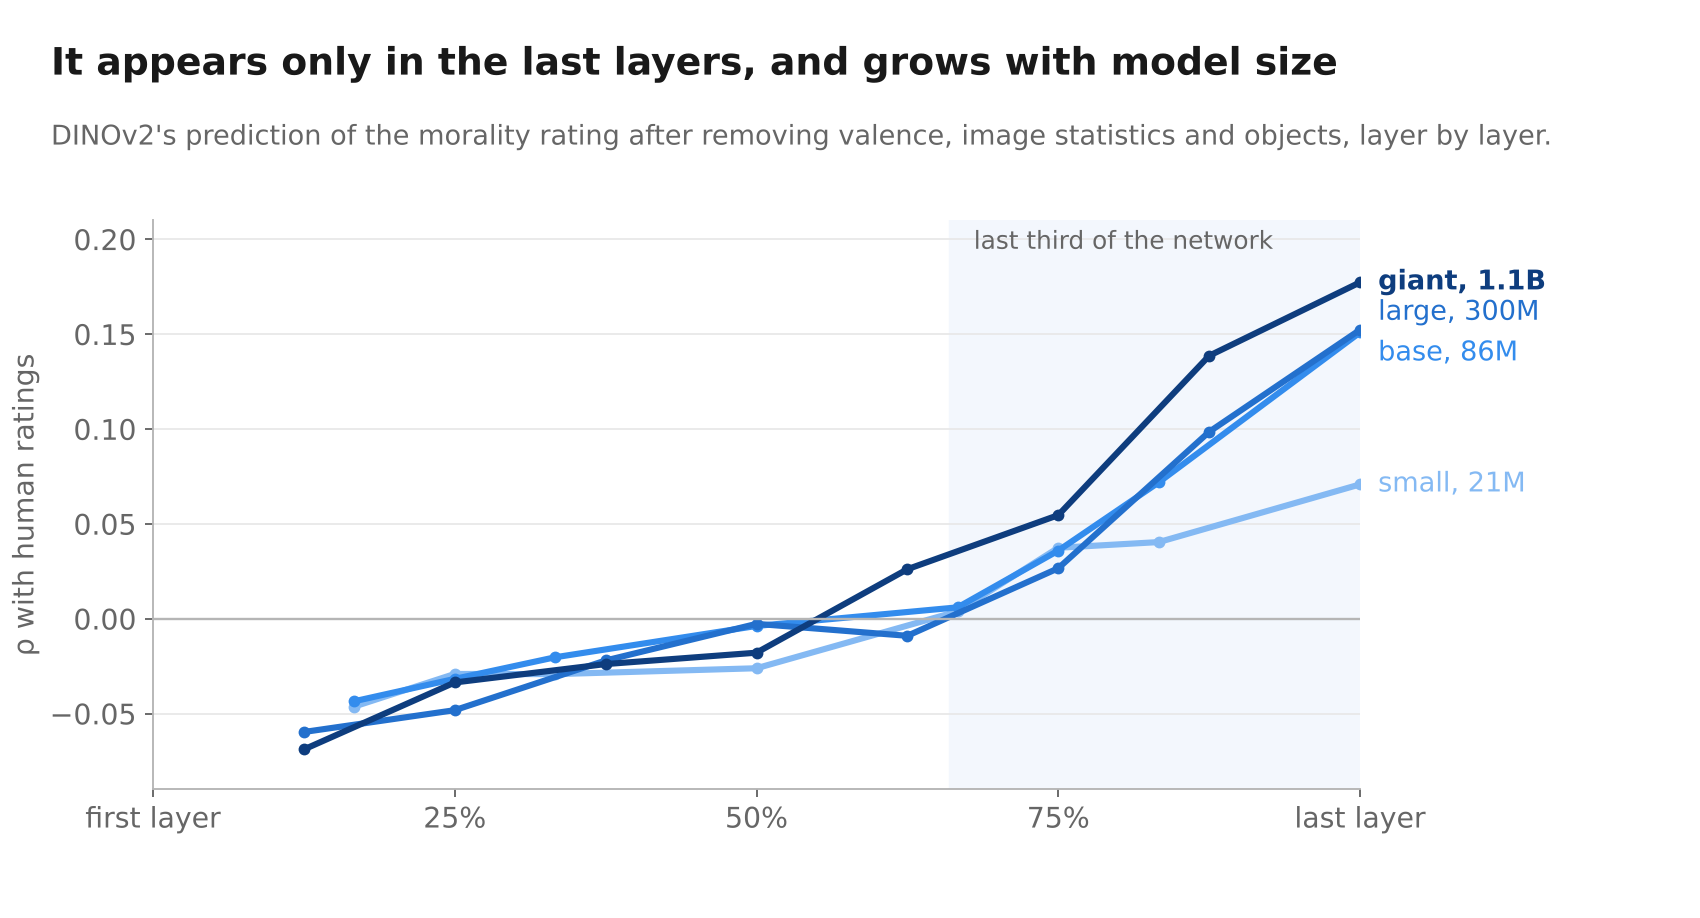
\includegraphics[width=0.8\linewidth]{fig5_depth_scale.png}
\caption{DINOv2's prediction of morality beyond valence, after removing low-level statistics, object scores and supervised features, by relative depth and model size.}\label{fig:depth}
\end{figure}

\begin{table}[ht]\centering\small
\begin{tabular}{lccc}\toprule
Target & Gain, S to g & 95\% CI & Minus object gain (95\% CI)\\\midrule
Morality after controls & 0.129 & 0.091--0.164 & 0.117 (0.080--0.152)\\
MBV after controls & 0.107 & 0.074--0.140 & 0.095 (0.061--0.128)\\
Valence after controls & 0.089 & 0.058--0.118 & 0.077 (0.047--0.106)\\
Object content (first component) & 0.013 & 0.005--0.022 & --\\\bottomrule
\end{tabular}
\caption{Best-layer gain in $\rho$ from the smallest to the largest DINOv2, paired bootstrap over images.}\label{tab:gain}
\end{table}

\section{Test 6: Do different models share the direction?}\label{sec:shared}

The Platonic Representation Hypothesis \cite{huh2024} holds that models trained on different data and objectives converge toward a shared picture of the world as they improve. If good versus bad is part of that picture, a caption-trained model (CLIP) and a vision-only model (DINOv2) should share it, more so as the models grow. All results here are against the human morality ratings.

\paragraph{6a. Agreement in both directions.} We fitted two linear maps on the unrated COCO photographs (512 principal components): one from DINOv2-g to CLIP, one from CLIP to DINOv2-g. DINOv2's morality probe, applied to CLIP features translated into DINOv2's space, predicts morality at $\rho=0.71$ (0.69--0.73), almost as well as on DINOv2's own features (0.74). For morality beyond valence the figures are 0.57 and 0.61. In the other direction, CLIP's probe applied to translated DINOv2 features reaches 0.62, against 0.87 on CLIP's own features. That gap fits CLIP holding more moral information than DINOv2 does.

\paragraph{6b. Agreement by depth and size.} For each DINOv2 size and five depths we ran a cross-validated version on SMID. Within each training split we fitted a DINOv2-to-CLIP map on the training images only, using their embeddings and no ratings. We also trained a morality probe on the CLIP embeddings of the same images. The CLIP probe was then applied to the translated DINOv2 embeddings of the held-out images. A high score means CLIP's morality direction is present inside DINOv2. In ViT-g it rises from 0.42 at 25\% depth to 0.54, 0.65 and 0.72 at 50, 75 and 90\%, and 0.73 at the last layer. At the last layer it grows from 0.64 in ViT-S to 0.73 in ViT-g (Table~\ref{tab:shared}, Figure~\ref{fig:shared}).

\paragraph{6c. Prominence.} A direction can be present yet minor. To check whether morality is one of the main axes of DINOv2's representation, we probed using only the first 10 principal components of each layer, which are found without labels. These 10 numbers predict morality at 0.43 in ViT-S and 0.56 in ViT-g, though not steadily in between. For comparison, the same 10 components of ViT-g predict edge density at 0.60 and brightness at 0.33.

\paragraph{6d. Overall similarity.} The mutual nearest-neighbour measure of Huh et al.\ \cite{huh2024} asks how often two models agree on each image's 10 most similar images. Between DINOv2 and CLIP it rises from about 0.02 at the first layer to 0.24--0.29 at the last layers, in the same layers where the moral signal appears. It increases from ViT-S (0.24) to ViT-B (0.28) and then levels off. The supervised ViT agrees with CLIP at 0.28.

\begin{table}[ht]\centering\small
\begin{tabular}{lcccc}\toprule
 & ViT-S & ViT-B & ViT-L & ViT-g\\\midrule
CLIP's morality direction in DINOv2 (last layer) & 0.642 & 0.692 & 0.714 & 0.732\\
CLIP's direction for morality beyond valence (last layer) & 0.550 & 0.588 & 0.590 & 0.605\\
Morality from the first 10 principal components (best layer) & 0.435 & 0.514 & 0.477 & 0.563\\
Mutual 10-NN agreement with CLIP (best layer) & 0.242 & 0.279 & 0.289 & 0.285\\\bottomrule
\end{tabular}
\caption{Shared structure between DINOv2 and CLIP, by DINOv2 size. The first three rows are Spearman $\rho$ with the human ratings.}\label{tab:shared}
\end{table}

\begin{figure}[ht]\centering
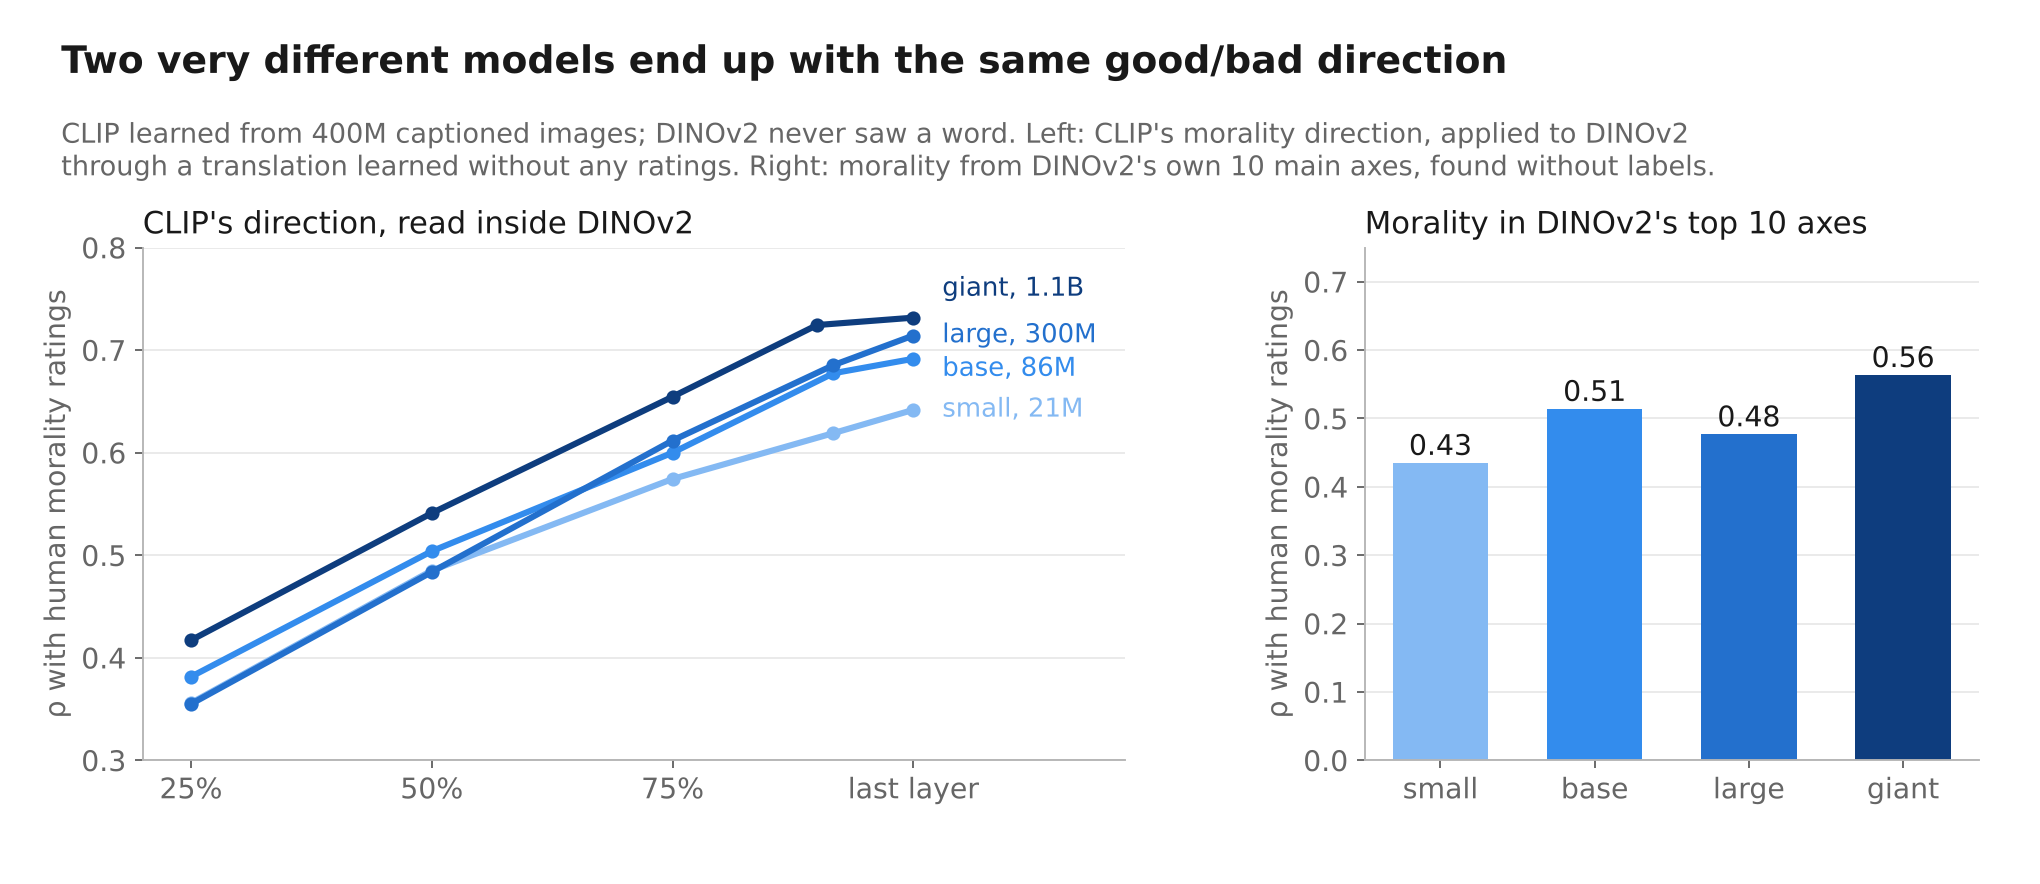
\includegraphics[width=0.95\linewidth]{fig6_shared_direction.png}
\caption{Left: CLIP's morality direction read inside DINOv2, by depth and size. Right: morality predicted from DINOv2's first 10 principal components only.}\label{fig:shared}
\end{figure}

\section{Discussion}

\paragraph{What we found.} DINOv2 never saw a label or a word, yet it orders photographs from morally bad to good much as people do. The ordering is not explained by image statistics or by the objects in the picture, and part of it reflects morality beyond pleasantness. Read in language, the direction separates virtue from vice, and helping and heroism from things that are merely pleasant. It appears late in the network and is stronger in larger models. Prior work found moral directions in language models \cite{schramowski2022,zou2023} and predicted SMID ratings from CLIP \cite{zhu2025}. What is new here is a model with no access to language, tested against shortcuts, and followed across depth, scale and a second model.

\paragraph{A shared concept?} The Natural Abstraction Hypothesis \cite{wentworth2021} proposes that some summaries of the world are useful enough for prediction that many different learners acquire them. The Platonic Representation Hypothesis \cite{huh2024} makes a similar claim about whole representations. If moral good versus bad is such a summary, three things should hold: models trained in very different ways agree on it, the agreement grows with capability, and it is prominent in a model's own structure rather than a faint direction only a probe can find. Test~6 supports all three. DINOv2's morality probe works almost as well on CLIP's translated features as on its own. CLIP's direction inside DINOv2 strengthens with depth and size. And the first 10 principal components of DINOv2 already carry much of the moral rating.

\paragraph{Why would an image-only model learn this?} DINOv2 is trained to give matching representations to different crops of the same photograph, so it must encode what stays the same across crops: what kind of scene it is and what is happening in it. In photographs of people, a large part of that is who is hurt, who is helping and what is likely to happen next. Those are close to what raters judge as good or bad. On this account the moral signal is part of understanding a scene well, which fits its appearing in the last layers, after objects, and growing with capacity while object information does not.

\paragraph{What this does not yet show.} The convergence evidence covers two models, not the many model families a real test of the hypothesis needs. Our translations are learned from paired images; an unpaired translation \cite{jha2025,tasker2026} would be a stricter test. And what the models share may be the structure of situations that human moral judgements track, rather than morality as such. Separating the two needs images in which the same visible situation carries different moral meaning.

\paragraph{Relevance to alignment.} If concepts tied to human values appear in capable models without being taught, they can be found and read out without labels, which helps interpretability and monitoring. The same mechanism means models inherit the moral categories, and the blind spots, of the images and judgements they learn from.

\section{Limitations}\label{sec:limits}
\begin{itemize}
\item \textbf{One dataset.} All ratings come from SMID and its rater sample. A second rated image set, such as OASIS \cite{kurdi2017}, would test generality.
\item \textbf{Distilled sizes.} DINOv2's ViT-S, B and L are distilled from ViT-g \cite{oquab2023}, so the size trend partly measures how much of the teacher a student keeps. Independently trained sizes would be a cleaner test.
\item \textbf{The strictest control.} After stacked linear and non-linear removal of the control features, morality beyond valence is no longer significant in DINOv2, though it is in CLIP. Because the supervised classifier in that control itself predicts the target, the control probably removes real signal as well, and we cannot tell how much.
\item \textbf{Probing.} Linear decodability does not mean the network uses the information \cite{belinkov2022,hewitt2019}. A causal test, such as editing representations along the direction, is future work.
\item \textbf{Not yet run.} A randomly initialised DINOv2 as a baseline.
\end{itemize}

\section{Reproducibility}
Code, result files and a Colab notebook are at \url{https://github.com/eliovi/moral_judgement_in_dinov2}. Feature extraction (\texttt{src/extract.py}) needs a GPU. Every test runs on CPU from the cached features, one script per test:\\ \texttt{e1\_probe\_layers.py} (Test 1), \texttt{e2\_shortcuts.py} (Test 2), \texttt{e3\_beyond\_valence.py} (Test 3),\linebreak \texttt{e4\_words.py} (Test 4), \texttt{e5\_depth\_scale.py} (Test 5) and \texttt{e6\_shared.py} (Test 6). The probe, statistics and cache layout are in \texttt{src/common.py}. Software: PyTorch, Hugging Face Transformers and scikit-learn \cite{pedregosa2011}.

\begin{thebibliography}{99}\small
\bibitem{alain2016} G.~Alain and Y.~Bengio. Understanding intermediate layers using linear classifier probes. arXiv:1610.01644, 2016.
\bibitem{belinkov2022} Y.~Belinkov. Probing classifiers: Promises, shortcomings, and advances. \emph{Computational Linguistics}, 48(1), 2022.
\bibitem{crone2018} D.~L.~Crone, S.~Bode, C.~Murawski and S.~M.~Laham. The Socio-Moral Image Database (SMID): A novel stimulus set for the study of social, moral and affective processes. \emph{PLOS ONE}, 13(1):e0190954, 2018. \href{https://doi.org/10.1371/journal.pone.0190954}{doi:10.1371/journal.pone.0190954}
\bibitem{deng2009} J.~Deng, W.~Dong, R.~Socher, L.-J.~Li, K.~Li and L.~Fei-Fei. ImageNet: A large-scale hierarchical image database. \emph{CVPR}, 2009.
\bibitem{dosovitskiy2021} A.~Dosovitskiy et al. An image is worth 16x16 words: Transformers for image recognition at scale. \emph{ICLR}, 2021. arXiv:2010.11929.
\bibitem{graham2013} J.~Graham, J.~Haidt, S.~Koleva, M.~Motyl, R.~Iyer, S.~P.~Wojcik and P.~H.~Ditto. Moral Foundations Theory: The pragmatic validity of moral pluralism. \emph{Advances in Experimental Social Psychology}, 47, 2013.
\bibitem{hewitt2019} J.~Hewitt and P.~Liang. Designing and interpreting probes with control tasks. \emph{EMNLP}, 2019. arXiv:1909.03368.
\bibitem{huh2024} M.~Huh, B.~Cheung, T.~Wang and P.~Isola. The Platonic Representation Hypothesis. \emph{ICML}, 2024. arXiv:2405.07987.
\bibitem{jha2025} R.~Jha, C.~Zhang, V.~Shmatikov and J.~X.~Morris. Harnessing the universal geometry of embeddings. arXiv:2505.12540, 2025.
\bibitem{kurdi2017} B.~Kurdi, S.~Lozano and M.~R.~Banaji. Introducing the Open Affective Standardized Image Set (OASIS). \emph{Behavior Research Methods}, 49, 2017.
\bibitem{lin2014} T.-Y.~Lin et al. Microsoft COCO: Common objects in context. \emph{ECCV}, 2014. arXiv:1405.0312.
\bibitem{oquab2023} M.~Oquab, T.~Darcet, T.~Moutakanni et al. DINOv2: Learning robust visual features without supervision. \emph{TMLR}, 2024. arXiv:2304.07193.
\bibitem{pedregosa2011} F.~Pedregosa et al. Scikit-learn: Machine learning in Python. \emph{JMLR}, 12, 2011.
\bibitem{radford2021} A.~Radford et al. Learning transferable visual models from natural language supervision. \emph{ICML}, 2021. arXiv:2103.00020.
\bibitem{schramowski2022} P.~Schramowski, C.~Turan, N.~Andersen, C.~A.~Rothkopf and K.~Kersting. Large pre-trained language models contain human-like biases of what is right and wrong to do. \emph{Nature Machine Intelligence}, 4(3), 2022. \href{https://doi.org/10.1038/s42256-022-00458-8}{doi:10.1038/s42256-022-00458-8}
\bibitem{tasker2026} Tasker, Betser, Gofer, Levi and Gilboa. The Universal Normal Embedding. arXiv:2603.21786, 2026.
\bibitem{wentworth2021} J.~Wentworth. Testing the Natural Abstraction Hypothesis: Project intro. \emph{LessWrong / AI Alignment Forum}, 2021. \url{https://www.lesswrong.com/posts/cy3BhHrGinZCp3LXE}
\bibitem{zhu2025} W.~Zhu, A.~Ramezani and Y.~Xu. Visual moral inference and communication. \emph{CogSci}, 2025. arXiv:2504.11473.
\bibitem{zou2023} A.~Zou et al. Representation engineering: A top-down approach to AI transparency. arXiv:2310.01405, 2023.
\end{thebibliography}
\end{document}
